%!TEX TS-program = lualatex
%!TEX encoding = UTF-8 Unicode

%\frame[plain]{ % When including a large figure or table, you don't want to have the bottom and the top of the slides.
%\frame[shrink]{ % If you want to include lots of text on a slide, use the shrink option.

\begin{frame}
    \frametitle{libguestfs}
    \begin{itemize}
        \item library and suite of utilities for offline FS access
        \item mature ecosystem, many useful utilities
        \item used for Simics-externfs
    \end{itemize}

\begin{center}
    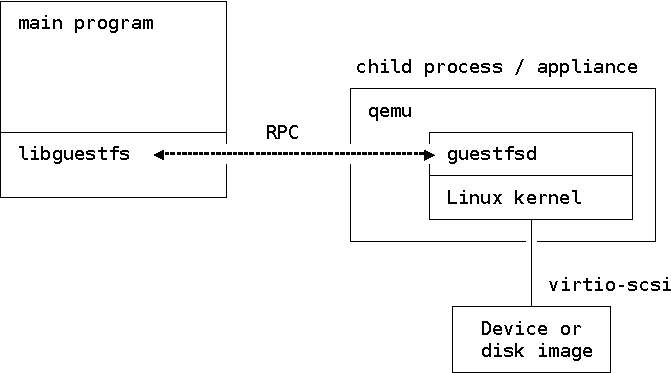
\includegraphics[width=.65\textwidth]{frames/img/libguestfs_arch}
\end{center}
    
    \note{
        \begin{itemize}
            \item library and suite of utilities for offline FS access
            \item conversion of physical or virtual to virtual, install OS
            \item runs a stripped down Linux appliance using libvirt and/or QEMU for FS-access
            \item quite some overhead, but the goal is to isolate the operations from the host
            \item mature ecosystem, many useful utilities (install OS, convert OS to other HV, tail etc.)
            \item used for Simics-externfs
        \end{itemize}
    }
\end{frame}